% SOURCE: 2026年辽宁省大学生物理实验竞赛设计报告 — 自选类创新作品 方向2（虚仿）
\documentclass[12pt,a4paper]{ctexart}

% ==== Layout ====
\usepackage[margin=1in]{geometry}
\setlength{\parindent}{2em}
\renewcommand{\baselinestretch}{1.25}

% ==== Fonts (auto-detected 2026-06-18) ====
\newcommand{\fontpath}{C:/Users/FengZhiHen/AppData/Local/Microsoft/Windows/Fonts/}
\setmainfont{Times New Roman}
\setCJKmainfont{simsun.ttc}[AutoFakeBold=2.5]
\setCJKsansfont{SimHei.ttf}[AutoFakeBold=1.5]
\setCJKmonofont{SimHei.ttf}[AutoFakeBold=1.5]

\setCJKfamilyfont{zhonghei}{SimHei.ttf}[AutoFakeBold=1.5]
\setCJKfamilyfont{zhongkai}{楷体_GB2312.TTF}[AutoFakeBold=2.0, Path=\fontpath]
\setCJKfamilyfont{zhongfang}{仿宋_GB2312.ttf}[AutoFakeBold=2.5, Path=\fontpath]
\setCJKfamilyfont{zhongxbs}{方正小标宋简.TTF}[Path=\fontpath]

\newcommand{\heitil}{\CJKfamily{zhonghei}}
\newcommand{\kaitil}{\CJKfamily{zhongkai}}
\newcommand{\fangsongl}{\CJKfamily{zhongfang}}
\newcommand{\xiaobiaosong}{\CJKfamily{zhongxbs}}

% ==== Packages ====
\usepackage{graphicx}
\usepackage{booktabs}
\usepackage{amsmath,amssymb}
\usepackage{bm}
\usepackage{hyperref}
\usepackage[section]{placeins}
\usepackage{flafter}
\usepackage{enumitem}
\usepackage{caption}
\usepackage{listings}
\usepackage{xcolor}
\usepackage{tabularx}
\usepackage{tikz}
\usetikzlibrary{arrows.meta, positioning, shapes.geometric, fit}

% ==== Float control ====
\setcounter{totalnumber}{5}
\renewcommand{\topfraction}{0.9}
\renewcommand{\textfraction}{0.1}

% ==== Graphics path ====
% 注意：此路径依赖 build.py 在 src/ 目录下运行 xelatex
% 若手动编译，需 cd 到 src/ 目录执行 xelatex
\graphicspath{{../figures/output/}}

% ==== Code listings ====
\lstset{
  basicstyle=\small\ttfamily,
  breaklines=true,
  frame=single,
  numbers=left,
  numberstyle=\tiny,
  language=Python,
}

% ==== Hyperref ====
\hypersetup{
    colorlinks=true,
    linkcolor=blue,
    citecolor=blue,
    urlcolor=blue,
}

\title{\xiaobiaosong 双摆非线性动力学虚拟仿真实验\\[0.5em] \large ——设计报告}
\date{\today}
\author{}

\begin{document}

\maketitle

\begin{abstract}
本设计报告详述了一个面向本科物理教学的\textbf{双摆非线性动力学虚拟仿真实验}系统的设计与实现。
该系统以平面理想双摆为物理模型，基于拉格朗日力学导出运动方程，自实现 RKF45 自适应步长积分引擎，
在 Web Worker 中并行求解 ODE 并通过 Transferable Float64Array 零拷贝传输结果。
系统提供探索、分析、实验、故事四种工作模式，构建“感知→分析→验证→创造”四层递进认知闭环。
核心技术栈包括 React 18 + TypeScript + Three.js + Web Audio API + Pyodide，
产出物为纯客户端、零后端依赖的自包含 HTML5 文件夹，支持离线运行。
本报告从物理原理、系统架构、数值方法、交互设计、结果验证等方面展开论述。
物理验证结果表明：小角度线性化偏差低于 0.8\%，单摆退化周期偏差低于 0.05\%，
1000 秒无阻尼仿真能量漂移仅为 0.38\%，为系统的物理正确性提供了量化背书。
本报告旨在为同类虚拟仿真教学资源的开发提供完整的技术参考。
\end{abstract}

\tableofcontents
\newpage

% ==== 章节 ====
% SOURCE: docs/比赛材料/开发目的.md + docs/比赛材料/设计原理与方法.md §引言
\section{选题意义与目标定位}

\subsection{混沌理论的教学价值与现状}

非线性动力学与混沌理论是 20 世纪物理学的三大革命性突破之一，与相对论和量子力学并列。
混沌揭示了确定性系统产生表观随机行为的深刻机制——这一发现从根本上改变了人类对“可预测性”的哲学理解。
然而，在国内本科物理课程体系中，混沌内容长期处于边缘地位：多数《大学物理》课程以线性振动（简谐运动、阻尼振动、受迫振动）为核心，
对非线性振动和混沌仅以“科普讲座”或“绪论末尾”形式简要提及，缺乏系统性教学支撑。

学生的典型认知障碍包括：(1) 将“决定论”与“可预测性”等同——认为既然微分方程唯一确定，则长期预测必为可行；
(2) 将“偶然性”与“不可预测性”混为一谈——无法区分量子力学的不确定性与经典混沌的初值敏感性。
这些概念混淆是混沌教学中的主要卡点，传统以文字描述和静态图片为主的教材呈现方式难以有效纠正。

\subsection{实体实验的固有瓶颈与数字资源的不足}

双摆是混沌教学的经典模型——仅两个自由度却能展现从周期运动到完全混沌的全谱系动力学行为。
但实体双摆实验面临多重困境：

\begin{enumerate}[label=(\arabic*), leftmargin=*]
  \item \textbf{加工精度要求苛刻}：转轴摩擦、空气阻力、轴承间隙会掩盖真实的混沌动力学行为，使实验现象偏离理论预期；
  \item \textbf{参数调节效率低下}：摆长、质量需物理拆装，无法实现“滑杆拖拽即生效”的即时反馈，而绘制一条完整分岔图需扫描数百个参数点，课堂时间内无法完成；
  \item \textbf{数据采集存在系统性偏差}：传感器精度、量化误差、机械摩擦损耗使测量结果与理论模型之间存在不可忽略的差距；
  \item \textbf{初始条件难以精确复现}：实验可重复性差，参数调试不当会掩盖混沌态中的周期窗口、拉长实验周期。
\end{enumerate}

另一方面，现有数字资源也未能填补空白：Flash/MP4 演示动画“只能看不能操作”，MATLAB/Python 离线脚本“需安装环境、调试代码，门槛高”。
多数仿真工具停留在现象演示层面，缺乏从“感知→分析→验证→创造”的完整认知路径，且商业软件授权复杂、成本高，不适合大规模课堂部署。

\subsection{本作品的目标定位}

本作品旨在提供一个\textbf{纯浏览器端、零安装门槛、离线可运行}的双摆非线性动力学虚拟仿真平台，
通过高精度数值积分引擎驱动实时物理仿真，以四层递进认知架构覆盖从入门感知到科研训练的完整教学需求。

具体目标包括：
\begin{enumerate}[label=(\arabic*), leftmargin=*]
  \item \textbf{以数值仿真替代实体实验}：自实现 RKF45 自适应步长积分引擎，在 Web Worker 中并行求解双摆 ODE，消除机械摩擦、传感器噪声和量化误差；
  \item \textbf{构建完整认知闭环}：设计探索（感知）、分析（理解）、实验（验证）、故事（展示）四种工作模式，使学生从直观感受混沌现象出发，逐步建立定量分析能力；
  \item \textbf{实现零门槛部署}：纯客户端架构，产出物为自包含 HTML5 文件夹，支持 \texttt{file://} 协议离线运行，可嵌入课程网站、拷入 U 盘、部署在教室一体机或科技馆终端；
  \item \textbf{纠正关键认知误区}：通过蝴蝶效应双视口对比器（$\delta\theta_1 = 10^{-6\circ}$）和时间反演双模式实验（精确/数值对比），直观展示“确定性但不可预测”的物理本质。
\end{enumerate}

\endinput

\clearpage
% SOURCE: docs/比赛材料/设计原理与方法.md §一–§二 + §五–§六
\section{物理原理}

\subsection{双摆系统定义}

本系统研究的物理对象为\textbf{平面理想双摆}（Planar Ideal Double Pendulum），其力学定义如下：

\begin{itemize}
  \item 两根质量不计的刚性杆，长度分别为 $L_1$、$L_2$；
  \item 两个质点 $m_1$、$m_2$ 分别固定于两杆末端；
  \item 上端支点固定于原点，系统在竖直平面（$xy$ 平面）内运动；
  \item 均匀重力场 $g$，方向竖直向下（$-y$ 方向）；
  \item 可选线性粘滞阻尼，阻尼力矩 $\tau_i = -b\,\dot{\theta}_i$（$i = 1,2$）。
\end{itemize}

选取两杆与竖直向下方向的偏角 $(\theta_1, \theta_2)$ 为广义坐标，逆时针为正方向。
以悬挂点为原点，$y$ 轴向上，笛卡尔坐标到广义坐标的映射为：

\begin{equation}
\begin{aligned}
  x_1 &= L_1 \sin\theta_1, \quad y_1 = -L_1 \cos\theta_1 \\
  x_2 &= x_1 + L_2 \sin\theta_2, \quad y_2 = y_1 - L_2 \cos\theta_2
\end{aligned}
\label{eq:kinematics}
\end{equation}

\subsection{拉格朗日方程与运动方程}

系统动能 $T$ 与势能 $V$ 为：

\begin{equation}
\begin{aligned}
  T &= \frac{1}{2}m_1 L_1^2 \dot{\theta}_1^2
     + \frac{1}{2}m_2\Bigl[L_1^2\dot{\theta}_1^2 + L_2^2\dot{\theta}_2^2
     + 2L_1 L_2\dot{\theta}_1\dot{\theta}_2\cos(\theta_2-\theta_1)\Bigr] \\[0.5em]
  V &= -(m_1+m_2)gL_1\cos\theta_1 - m_2 g L_2 \cos\theta_2
\end{aligned}
\label{eq:energy}
\end{equation}

拉格朗日函数 $L = T - V$，代入欧拉--拉格朗日方程：

\begin{equation}
  \frac{d}{dt}\frac{\partial L}{\partial \dot{\theta}_i} - \frac{\partial L}{\partial \theta_i} = -b\,\dot{\theta}_i, \quad i = 1,2
\label{eq:euler_lagrange}
\end{equation}

引入角度差 $\delta = \theta_2 - \theta_1$，经矩阵求逆，得到角加速度的显式表达式——\textbf{即本系统 ODE 右端函数的实现依据}：

\begin{equation}
\boxed{
\begin{aligned}
\ddot{\theta}_1 &= \frac{m_2 L_1 \dot{\theta}_1^2 \sin\delta\cos\delta
                  + m_2 g \sin\theta_2 \cos\delta
                  + m_2 L_2 \dot{\theta}_2^2 \sin\delta
                  - (m_1+m_2)g\sin\theta_1}
                  {L_1\bigl[m_1 + m_2\sin^2\delta\bigr]} - b\,\dot{\theta}_1 \\[1.5em]
\ddot{\theta}_2 &= \frac{-m_2 L_2 \dot{\theta}_2^2 \sin\delta\cos\delta
                  + (m_1+m_2)\bigl(g\sin\theta_1\cos\delta
                  - L_1\dot{\theta}_1^2\sin\delta
                  - g\sin\theta_2\bigr)}
                  {L_2\bigl[m_1 + m_2\sin^2\delta\bigr]} - b\,\dot{\theta}_2
\end{aligned}
}
\label{eq:ode_system}
\end{equation}

其中分母 $m_1 + m_2\sin^2\delta$ 在极端参数组合下可能趋近于零，代码中以 \texttt{DENOM\_EPSILON = 1e-12} 做近零保护。

\subsection{退化验证}

上述运动方程在两个经典极限情形下退化：

\textbf{单摆退化}（$m_2 \to 0$）：分母趋近 $m_1$，$\ddot{\theta}_1 \to -(g/L_1)\sin\theta_1$，退化为标准单摆方程，
其小角度周期 $T_0 = 2\pi\sqrt{L_1/g}$。

\textbf{小角度线性化}（$|\theta_1|,|\theta_2| \ll 1$，$b = 0$）：在 $(0,0)$ 处 Taylor 展开至一阶，得到耦合线性振动系统，存在两个正则模（Normal Modes）。
正则模频率为：
\begin{equation}
  \omega^2_{\pm} = \frac{g}{2}\left[\frac{m_1+m_2}{m_1}\left(\frac{1}{L_1}+\frac{1}{L_2}\right)
                   \pm \sqrt{\left(\frac{m_1+m_2}{m_1}\right)^2\left(\frac{1}{L_1}+\frac{1}{L_2}\right)^2
                   - \frac{4(m_1+m_2)}{m_1 L_1 L_2}}\,\right]
\label{eq:normal_modes}
\end{equation}

上述退化情形均已编码为物理验证套件的自动化测试场景，确保 ODE 实现的物理正确性。

\subsection{混沌的数学定义：Lyapunov 指数}

混沌系统最核心的量化特征是其对初值的指数级敏感性。\linebreak
对于状态向量 $\mathbf{x} = (\theta_1,\dot{\theta}_1,\theta_2,\dot{\theta}_2)^T$，定义最大 Lyapunov 指数（MLE）：

\begin{equation}
  \lambda_{\max} = \lim_{t\to\infty}\lim_{\delta\mathbf{x}_0\to 0}\,\frac{1}{t}\ln\frac{\|\delta\mathbf{x}(t)\|}{\|\delta\mathbf{x}_0\|}
\label{eq:lyapunov_def}
\end{equation}

其中 $\delta\mathbf{x}(t)$ 是初始微扰 $\delta\mathbf{x}_0$ 随时间的演化。$\lambda_{\max} > 0$ 是混沌的充分条件。

本系统采用 Benettin 算法估算 MLE：并行积分参考轨线与扰动轨线，每隔固定周期 $\tau$ 测量扰动增长倍数并重新归一化扰动方向，
最终 $\lambda_{\max} = \frac{1}{N\tau}\sum_{k=1}^{N}\ln(d_k/\delta_0)$。
离线预计算脚本在参数空间 $(L_2/L_1,\;\theta_{1,0})$ 上生成 $100 \times 100$ 网格的 MLE 矩阵，为前端的 Lyapunov 热力图提供数据源。

\subsection{时间反演与蝴蝶效应}

双摆的哈密顿量在无阻尼条件下可逆——若以 $(\theta_1, \theta_2, -\dot{\theta}_1, -\dot{\theta}_2)$ 为初值，
理论轨迹应沿原路径反向返回。但在数值仿真中，浮点舍入误差（$\sim 10^{-16}$）被正 Lyapunov 指数放大约 $e^{\lambda t}$ 倍，
导致数值反演轨迹逐渐偏离原路径。这一现象构成了“哈密顿可逆性 vs 数值不可逆性”的核心教学命题。

蝴蝶效应本质上是同一数学事实的另一面：两个仅相差 $\Delta\theta_1(0) \approx 10^{-6\circ}$ 的初始条件，
其轨迹差异 $\|\Delta\mathbf{x}(t)\|$ 随时间指数增长，在李雅普诺夫时间 $\tau_L = 1/\lambda_{\max}$ 尺度上变得宏观可见。
本系统的蝴蝶效应对比器以双 Worker 并行积分、双 Viewport 并排渲染的方式，将此抽象概念转化为直观的视觉叙事。

\endinput

\clearpage
% SOURCE: docs/比赛材料/设计原理与方法.md §三 + docs/双摆混沌实验室-技术栈设计.md
\section{系统设计与实现}

\subsection{分层架构设计}

本系统采用前端五层 Clean Architecture，自底向上为（图\ref{fig:architecture}）：

\begin{description}[leftmargin=*, itemsep=0.5em]
  \item[Domain 层] 实体/值对象/领域服务：ODE 右端函数、三种积分器\linebreak
                    （RKF45/VelocityVerlet/Euler）、能量与漂移计算器、庞加莱截面穿越检测、力分量计算器。
  \item[Application 层] 无状态用例：BootSequence、SaveSnapshot、ExportData、RunValidation 等。
  \item[Infrastructure 层] 端口实现：Worker 调度器与批量积分管线、IndexedDB 缓存管理、
                           音频合成引擎（Web Audio API）、PDF/CSV/PNG 导出器、Pyodide 桥接。
  \item[ViewModel 层] Zustand Store + 自定义 Hooks：管理仿真状态、模式切换、快照管理、多视图联动。
  \item[View 层] React 组件（纯渲染，不含业务逻辑）：3D 场景（R3F）、2D 图表（D3.js Canvas）、
                 控制面板（shadcn/ui）、代码编辑器（CodeMirror 6）。
\end{description}

依赖方向铁律：上层可依赖下层，反向绝对禁止。View 层不直接调用 API 或 Worker，全部通过 ViewModel 层 Hooks 间接消费数据。

\begin{figure}[htbp]
  \centering
  \fbox{%
    \begin{minipage}{0.85\textwidth}
      \vspace{1em}
      \begin{center}
        \textbf{五层 Clean Architecture}\\[0.5em]
        \small
        \begin{tabularx}{\linewidth}{|c|>{\centering\arraybackslash}p{5cm}|X|}
          \hline
          \textbf{层级} & \textbf{技术实现} & \textbf{职责} \\
          \hline
          View & React + R3F + D3.js + shadcn/ui & 纯渲染、用户交互 \\
          \hline
          ViewModel & Zustand Store + Hooks & 状态管理、业务编排 \\
          \hline
          Infrastructure & Worker 调度器、IndexedDB、Audio API、Pyodide & 端口实现 \\
          \hline
          Application & 无状态用例 (Boot/Save/Export/Validate) & 业务流程 \\
          \hline
          Domain & ODE 右端函数、积分器、力计算器 & 纯领域逻辑 \\
          \hline
        \end{tabularx}
      \end{center}
      \vspace{0.5em}
    \end{minipage}
  }
  \caption{系统五层架构示意图}
  \label{fig:architecture}
\end{figure}

\subsection{仿真数据管线}

仿真数据管线是本系统的核心基础设施，其设计目标为：高频积分不阻塞 UI、零拷贝数据传输、历史数据可回溯（图\ref{fig:pipeline}）。

\begin{figure}[htbp]
  \centering
  \fbox{%
    \begin{minipage}{0.85\textwidth}
      \vspace{0.8em}
      \begin{center}
        \textbf{仿真数据流}\\[0.5em]
        \begin{tabular}{c c c c c}
          ODE 积分器 & $\xrightarrow{\text{写入}}$ & Float64Array 池 & $\xrightarrow{\text{Transferable}}$ & 主线程 Zustand \\
          (Worker) & & (10 $\times$ 4000 元素) & & (Store) \\[1em]
          & & & & $\downarrow$ \\[0.5em]
          & & & & \shortstack{R3F 3D 场景 \\ D3.js 2D 图表 \\ Web Audio 声音化}
        \end{tabular}
      \end{center}
      \vspace{0.5em}
    \end{minipage}
  }
  \caption{仿真数据管线——从 ODE 积分到多视图渲染}
  \label{fig:pipeline}
\end{figure}

关键设计要点：

\begin{enumerate}[label=(\arabic*), leftmargin=*]
  \item \textbf{Web Worker 隔离}：ODE 积分在独立线程中执行，主线程永不阻塞，确保 3D 渲染维持在 60 fps；
  \item \textbf{Transferable 零拷贝}：\texttt{Float64Array} 通过 \texttt{postMessage} 的 Transferable 机制传输，
       所有权转移而非内存复制，避免高频 GC 抖动。池化设计（10 块 $\times$ 4000 元素 $\approx$ 320 KB）覆盖 2 秒轨迹缓冲；
  \item \textbf{批量积分与预取}：Worker 以 10 帧批次（\texttt{FRAMES\_PER\_BATCH}）为单位积分，
       预取阈值 \texttt{BATCH\_PREFETCH\_THRESHOLD = 5} 触发下一批次的异步准备，确保缓冲区永不枯竭；
  \item \textbf{环形缓冲区 历史存储}：容量 6000 帧（= 100 s @ 60 fps），循环覆盖，O(1) 写入与随机访问，
       作为时间反演回放与历史回溯的数据源。
\end{enumerate}

\subsection{数值积分方法}

本系统实现了三种积分器，以策略模式（Strategy Pattern）组织，通过 \texttt{IIntegrator} 契约接口统一调用。

\subsubsection{RKF45 自适应积分器（默认）}

采用 Fehlberg 4(5) 嵌入对，Butcher 表系数直接编码。核心特性：

\begin{itemize}
  \item \textbf{自适应步长控制}：每子步计算 4 阶与 5 阶估计的差值作为误差估计，以容差 $\text{tol} = 10^{-7}$ 为标准动态调整步长；
  \item \textbf{步长坍缩回退}：当误差持续超标导致 $h < 10^{-10}$ 时，自动退化为 Euler 子步避免死循环；
  \item \textbf{方向感知}：支持正向（$dt > 0$）与反向（$dt < 0$）积分，为时间反演实验提供数值基础。
\end{itemize}

RKF45 在 $\Delta t = 1/60\,\mathrm{s}$ 标称步长下，1000 s 仿真能量漂移控制在 $0.5\%$ 以下。

\subsubsection{Velocity Verlet 积分器}

Velocity Verlet 是一种辛积分器变体。需要特别指出：其辛性严格依赖于正则坐标 $(q, p)$ 的使用。
本系统以 $(\theta, \dot{\theta})$ 为状态变量（而非正则动量 $p = \partial L/\partial \dot{\theta}$），
因此 Velocity Verlet 在此并非严格辛（symplectic）的。实验中学生可观察到其长时能量漂移甚至可能劣于 RKF45——这本身构成一个重要的教学点。

\subsubsection{显式 Euler（教学对照）}

局部截断误差仅 $O(\Delta t^2)$。对于混沌双摆，数秒内即导致能量发散。保留此积分器作为教学对照案例，让学生直观体会低阶方法的局限性。

\subsection{核心技术栈}

\begin{table}[htbp]
  \centering
  \caption{核心技术栈一览}
  \label{tab:tech_stack}
  \begin{tabularx}{\textwidth}{l l X}
    \toprule
    \textbf{维度} & \textbf{技术} & \textbf{用途} \\
    \midrule
    语言/框架 & TypeScript 5.6 + React 18.3 & 前端 UI 与状态管理 \\
    构建工具 & Vite 5.4 & 开发/构建/自包含产物输出 \\
    3D 渲染 & Three.js 0.184 + R3F 8.17 + drei 9.114 & 实时 3D 场景、能量景观曲面、力矢量 \\
    2D 图表 & D3.js 7.x（按需模块） & 分岔图、热力图、庞加莱截面散点图 \\
    状态管理 & Zustand 4.5 & 全局状态与多视图联动 \\
    ODE 求解 & 自实现 RKF45/VelocityVerlet/Euler & Web Worker 常驻积分 \\
    音频合成 & Web Audio API（原生） & 混沌声音化引擎 \\
    Python 沙箱 & Pyodide 0.26 + CodeMirror 6 & 浏览器内 Python 可编程 \\
    样式 & Tailwind CSS 3.x + shadcn/ui & 原子化 CSS + 无障碍组件 \\
    测试 & Vitest + Testing Library & 单元测试 + 物理回归测试 \\
    \bottomrule
  \end{tabularx}
\end{table}

\subsection{代码归属说明}

按竞赛要求，明确区分已有函数、引用代码与自写代码：

\begin{table}[htbp]
  \centering
  \small
  \caption{代码归属分类}
  \label{tab:code_ownership}
  \begin{tabularx}{\textwidth}{l X}
    \toprule
    \textbf{类别} & \textbf{内容} \\
    \midrule
    \textbf{自主编写} &
    运动方程右端函数（\texttt{derivatives.ts}）；三种积分器（RKF45 / Velocity Verlet / Euler）；
    Worker 调度器与批量积分管线；Command Bus 通信协议；环形缓冲区存储（容量 6000 帧）；
    能量监控模块（含投影校正与漂移告警）；运动尾迹缓冲与颜色映射着色；
    蝴蝶效应双 Worker 同步控制；时间反演状态机与漂移计算；
    力分量计算器（支持笛卡尔 / 极坐标 / 自然坐标三坐标系切换）；
    物理验证三项自动化测试；庞加莱截面穿越检测（线性插值 + 二分定位）；
    分岔图与 Lyapunov 热力图的 Canvas 渲染引擎 \\
    \midrule
    \textbf{算法引用} &
    RKF45 Butcher 表系数（Fehlberg 嵌入对）；Benettin 最大 Lyapunov 指数估计；
    Modified Gram-Schmidt 正交归一化 \\
    \midrule
    \textbf{第三方库} &
    React 18（UI 框架）；Three.js / R3F / drei（3D 渲染）；
    D3.js（2D 图表缩放与坐标变换）；Zustand（状态管理）；
    CodeMirror 6（代码编辑器）；Web Audio API（浏览器原生音频）；
    Pyodide v0.26.1（Python WASM 运行时）；Tailwind CSS + shadcn/ui（样式系统）；
    jsPDF（PDF 报告生成） \\
    \bottomrule
  \end{tabularx}
\end{table}

\subsection{仿真流程}

系统仿真主循环的执行流程如图\ref{fig:sim_flowchart}所示。

\begin{figure}[htbp]
  \centering
  \begin{tikzpicture}[
    node distance=1.2cm and 1.8cm,
    box/.style={rectangle, draw, rounded corners=3pt, minimum width=5cm, minimum height=0.8cm, align=center, font=\small},
    decision/.style={diamond, draw, aspect=2, minimum width=3.5cm, minimum height=1cm, align=center, font=\small},
    arrow/.style={->, >=Stealth, thick},
  ]
    % Nodes
    \node[box] (init) {主线程创建 Worker + 初始化 Float64Array 池};
    \node[box, below=of init] (param) {用户调整参数（滑块 / 数值输入）};
    \node[box, below=of param, fill=blue!8] (batch) {Worker 批量积分 10 帧 \\(RKF45, $\Delta t = 1/60$ s)};
    \node[box, below=of batch, fill=green!8] (transfer) {Transferable postMessage \\(Float64Array 零拷贝传输)};
    \node[box, below=of transfer] (store) {主线程写入 Zustand Store};
    \node[box, below=of store, fill=yellow!8, minimum height=1.2cm] (render) {多视图同步渲染：\\R3F 3D 场景 + D3.js 图表 + Web Audio 声音化};
    \node[box, below=of render] (ring) {环形缓冲区追加历史帧（容量 6000 = 100 s）};
    \node[decision, below=of ring] (check) {缓冲区消耗 \\$\leq 5$ 帧？};
    \node[box, right=of check, xshift=4cm, fill=orange!10] (prefetch) {Worker 异步预取\\下一批次数据};

    % Arrows
    \draw[arrow] (init) -- (param);
    \draw[arrow] (param) -- (batch) node[midway, right, font=\footnotesize, align=left] {连续参数即时更新\\初始条件释放时触发};
    \draw[arrow] (batch) -- (transfer);
    \draw[arrow] (transfer) -- (store);
    \draw[arrow] (store) -- (render);
    \draw[arrow] (render) -- (ring);
    \draw[arrow] (ring) -- (check);
    \draw[arrow] (check) -- node[above, font=\footnotesize] {是} (prefetch);
    \draw[arrow] (prefetch.north) -- ++(0, 2.5) -| ([xshift=2cm]batch.east) -- (batch.east);
    \draw[arrow] (check.west) -- ++(-1.8,0) |- (batch.west);

  \end{tikzpicture}
  \caption{仿真主循环流程图}
  \label{fig:sim_flowchart}
\end{figure}

各步骤具体说明如下：

\begin{enumerate}[label=步骤 \arabic*:, leftmargin=*]
  \item \textbf{初始化}：主线程创建 Web Worker 实例，初始化 Float64Array 池（10 块 $\times$ 4000 元素）。
       Worker 加载 ODE 右端函数和积分器，等待启动指令；
  \item \textbf{参数变更}：用户通过滑块/数值输入修改物理参数。
       连续参数（$m, L, g, b$）即时推送至 Worker 更新 ODE 系数；
       初始条件参数（$\theta, \dot{\theta}$）在释放滑块时触发 Worker Reset + 清空尾迹；
  \item \textbf{批量积分}：Worker 每批次积分 10 帧（$\Delta t = 1/60$ s），
       结果写入从池中获取的 Float64Array，通过 Transferable postMessage 发送至主线程；
  \item \textbf{多视图同步}：主线程接收轨迹缓冲，写入 Zustand Store。React 调度器同步触发：
       (a) R3F 更新摆臂旋转、球位置、尾迹追加；(b) D3.js Canvas 更新相空间图/能量曲线；
       (c) Web Audio API 更新振荡器频率与音色；(d) 环形缓冲区追加历史帧；
  \item \textbf{预取判断}：当缓冲区消耗至 5 帧以下时，主线程向 Worker 发送预取命令，
       Worker 异步准备下一批次数据，确保缓冲区永不枯竭；
  \item \textbf{缓冲归还}：渲染完成后，Float64Array 归还至池，等待下一次分配。
\end{enumerate}

\subsection{交互设计逻辑}

系统包含四种工作模式，通过键盘数字键 1--4 一键切换，模式切换时仿真不中断，确保分析工具读取的是连续的运动数据：

\begin{table}[htbp]
  \centering
  \caption{四种工作模式与认知层级对应}
  \label{tab:modes}
  \begin{tabularx}{\textwidth}{c c l X}
    \toprule
    \textbf{快捷键} & \textbf{模式} & \textbf{认知层} & \textbf{核心功能} \\
    \midrule
    1 & 探索 & 感知 & 3D 实时渲染、参数拖拽调节、运动尾迹、声音化、蝴蝶效应分屏、时间反演 \\
    2 & 分析 & 理解 & Lyapunov 热力图、分岔图、庞加莱截面、能量监控面板 \\
    3 & 实验 & 验证 & 物理验证套件（三项标准）、受力拆解视图、Python 可编程沙箱 \\
    4 & 故事 & 展示 & 7 阶段自动演示、电影式字幕讲解、点击打断恢复手动控制 \\
    \bottomrule
  \end{tabularx}
\end{table}

\textbf{参数分类响应策略}：系统管理 10 个物理参数，采用分类响应策略以平衡即时反馈与计算效率：

\begin{itemize}
  \item \textbf{连续参数}（$m_1, m_2, L_1, L_2, g, b$）：拖拽滑块即时生效，仅更新 Worker 中的 ODE 系数，不重启积分状态；
  \item \textbf{初始条件参数}（$\theta_1, \dot{\theta}_1, \theta_2, \dot{\theta}_2$）：拖拽时在 3D 场景中半透明预览摆杆的新位置，
       释放滑块时才触发 Worker Reset 并清空尾迹——避免拖动过程中产生大量无效历史帧。
\end{itemize}

\textbf{响应式布局}：系统适配桌面（三栏：控制面板 | 3D 场景 | 图表面板）、平板（底部抽屉式控制面板）、手机（单栏聚焦 3D 场景，折叠高级功能）三类设备，
通过 Tailwind CSS 断点与 ResizeObserver 动态调整布局与渲染质量。

\endinput

\clearpage
% SOURCE: docs/比赛材料/参赛材料准备清单.md + 项目介绍-面向小组.md §四–§八
\section{使用方法}

\subsection{系统启动}

本系统为纯客户端 Web 应用，使用时无需安装任何软件或配置运行环境。获取方式为自包含 HTML5 离线文件夹，
双击 \texttt{index.html} 即可在浏览器中运行，无需网络连接或本地服务器。

首屏加载约 3--5 秒（取决于设备性能），期间显示加载动画。加载完成后，系统以默认参数自动启动双摆仿真，
3D 场景淡入呈现。

\subsection{探索模式——感知混沌}

探索模式（快捷键 \textbf{1}）是系统的默认入口，提供最直观的双摆交互体验：

\begin{itemize}
  \item \textbf{3D 场景操作}：鼠标左键拖拽旋转视角，滚轮缩放，右键平移。右上角视角预设按钮支持三视角一键切换：
       “实验员视角”（正面平视）、“上帝视角”（斜上方俯视）、“混沌视角”（自动缓慢旋转）；
  \item \textbf{运动尾迹}：摆球后方拖曳的彩色尾迹以颜色编码速度——蓝色（静止）→ 绿色 → 黄色 → 红色（高速），
       粗细随摆球速度动态变化。尾迹可在“显示选项”面板中切换开关或调整持久度；
  \item \textbf{参数调节}：左侧参数面板提供 10 个物理参数的滑块与数值输入双模式。
       参数分为两组——连续参数（质量、摆长、重力加速度、阻尼）和初始条件参数（角度、角速度）。
       参数的具体范围与默认值见表\ref{tab:params}；
  \item \textbf{声音化引擎}：点击底部声音开关按钮（需用户手势激活 AudioContext），
       系统将摆的运动实时转化为声音。上摆角度映射音高（$\theta_1 \to 220 + |\dot{\theta}_2| \times 200\;\mathrm{Hz}$），
       两摆夹角映射和声（纯五度 = 3:2 频率比；混沌态混入白噪声）；
  \item \textbf{蝴蝶效应对比器}：点击“蝴蝶效应”按钮，界面切换为左右并排的双 Viewport 布局。
       左侧金色摆 A 与右侧紫色摆 B 初始角度仅差 $10^{-6\circ}$，由两个独立 Worker 同步积分。
       分离度超过 90° 时触发脉冲提示，直观展示初值敏感性的指数放大效应；
  \item \textbf{时间反演实验}：点击“时间反演”按钮，可选择“精确反演”模式（直接回放 RingBuffer 历史帧，
       零误差回溯）或“数值反演”模式（Worker 以 $-dt$ 重新积分 ODE，因浮点误差被混沌指数放大而逐渐偏离原路径）。
       底部 Canvas 实时绘制漂移距离曲线，配合三阶段叙事提示（重合期 $\to$ 分离期 $\to$ 发散期）。
\end{itemize}

\begin{table}[htbp]
  \centering
  \caption{物理参数范围与默认值}
  \label{tab:params}
  \begin{tabularx}{\textwidth}{l c c c l}
    \toprule
    \textbf{参数} & \textbf{符号} & \textbf{范围} & \textbf{默认值} & \textbf{单位} \\
    \midrule
    上摆质量 & $m_1$ & 0.1 -- 5.0 & 1.0 & kg \\
    下摆质量 & $m_2$ & 0.1 -- 5.0 & 1.0 & kg \\
    上摆杆长 & $L_1$ & 0.1 -- 3.0 & 1.0 & m \\
    下摆杆长 & $L_2$ & 0.1 -- 3.0 & 1.0 & m \\
    上摆初始角度 & $\theta_1(0)$ & $-\pi$ -- $\pi$ & 2.094 ($120^\circ$) & rad \\
    上摆初始角速度 & $\dot{\theta}_1(0)$ & $-10.0$ -- $10.0$ & 0.0 & rad/s \\
    下摆初始角度 & $\theta_2(0)$ & $-\pi$ -- $\pi$ & $-1.047$ ($-60^\circ$) & rad \\
    下摆初始角速度 & $\dot{\theta}_2(0)$ & $-10.0$ -- $10.0$ & 0.0 & rad/s \\
    重力加速度 & $g$ & 0.1 -- 20.0 & 9.81 & m/s$^2$ \\
    阻尼系数 & $b$ & 0.0 -- 2.0 & 0.0 & s$^{-1}$ \\
    \bottomrule
  \end{tabularx}
\end{table}

\subsection{分析模式——理解混沌}

分析模式（快捷键 \textbf{2}）提供定量分析工具，帮助学生从“观看”走向“分析”：

\begin{itemize}
  \item \textbf{Lyapunov 指数热力图}：在参数空间 $(L_2/L_1,\;\theta_{1,0})$ 上显示 $100 \times 100$ 网格的彩色热力图。
       红色区域（$\lambda_{\max} > 0$）对应混沌参数区，蓝色区域（$\lambda_{\max} \approx 0$）对应规则运动区。
       悬停任意单元格可查看 MLE 精确值；点击单元格可将对应参数组合一键注入仿真 Store，
       自动切换到探索模式观看该参数下的 3D 双摆运动——实现“从理论图谱到直观运动”的无缝跳转；
  \item \textbf{分岔图}：以 $\theta_{1,0}$ 为控制参数横轴，纵轴为稳态阶段 $\theta_2(t)$ 的局部极大值集合。
       周期运动对应有限个孤立点，混沌运动对应雾状散点带。支持 D3.js 缩放（框选放大）和竖直游标联动当前仿真参数；
  \item \textbf{庞加莱截面}：选取截面 $\theta_1 = 0$，穿越方向 $\dot{\theta}_1 > 0$（默认，可配置）。
       Worker 实时检测穿越事件并以线性插值定位精确穿越点，Canvas 2D 动态生长散点图，
       新点以 $\alpha$ 渐变加入，自动截断至 10,000 点以防止性能退化；
  \item \textbf{能量监控面板}：实时显示动能 $K$、势能 $V$、总机械能 $E = K + V$ 的时间曲线。
       能量相对漂移 $\eta(t) = |E(t)-E(0)|/|E(0)|$ 持续监控——$\eta > 0.5\%$ 时触发告警锁存（需用户手动清除），
       长时间仿真（$\geq$ 5 分钟）自动触发能量投影校正。
\end{itemize}

\subsection{实验模式——验证混沌}

实验模式（快捷键 \textbf{3}）提供物理正确性的自动化验证与高级分析工具：

\begin{itemize}
  \item \textbf{物理验证套件}：三项标准验证一键运行，每项拥有独立四项状态机
       （idle $\to$ running $\to$ passed $|$ failed）：
       \begin{enumerate}[label=(\alph*), leftmargin=*]
         \item \textbf{小角度线性化}：设置 $\theta_1 \approx 3^\circ,\;\theta_2 \approx 2^\circ$，
              对比 RKF45 数值解与线性化解析解的偏差，断言 $< 2\%$；
         \item \textbf{单摆退化}：设置 $m_2 \to 0$，测量摆动周期，断言与 $T_0 = 2\pi\sqrt{L_1/g}$ 偏差 $< 1\%$；
         \item \textbf{能量守恒}：关闭阻尼，运行 1000 s 仿真，断言能量相对漂移 $< 0.5\%$。
       \end{enumerate}
       全部通过显示绿色徽章，不通过自动诊断可能原因（步长过大 / 积分器精度不足 / 阻尼未关闭）；
  \item \textbf{受力拆解视图}：在 3D 场景中叠加矢量箭头，实时显示重力、上摆拉力、下摆拉力、切向惯性力、法向惯性力的方向与大小。
       支持笛卡尔坐标、极坐标、自然坐标三种坐标系切换；
  \item \textbf{Python 可编程沙箱}：点击“Lab 模式”，加载 Pyodide（浏览器内 Python 运行时）与 CodeMirror 6 编辑器。
       系统提供三个预设模板（弹簧摆 / 受迫摆 / 磁力摆）作为起点。用户修改运动方程后点击“运行”，
       Pyodide 调用 SciPy \texttt{solve\_ivp} 求解，结果通过 JsProxy 转换为 Float64Array 注入 3D 场景。
       代码执行超时（5 s）自动中断，Python 异常解析行号后映射为中文错误提示。
\end{itemize}

\subsection{故事模式——展示混沌}

故事模式（快捷键 \textbf{4}）为自动演示模式，适用于课堂展示或答辩场景。系统按预编排的 7 个阶段自动推进
（总时长约 3 分 30 秒），每阶段包含：参数渐变过渡（lerp）、相机程序化运动、电影式字幕淡入淡出、关键按钮脉冲高亮。
用户点击任意位置可暂停自动流程并恢复手动控制。

\subsection{辅助功能}

\begin{itemize}
  \item \textbf{状态快照}：点击快照按钮保存当前完整仿真状态（含参数、状态向量、尾迹数据和 64px 缩略图）至 IndexedDB，
       最多保留 50 个快照。快照卡片排列展示，点击恢复对应状态。支持双快照参数差异对比；
  \item \textbf{历史回放}：底部时间轴 Slider 基于 RingBuffer（100 s 历史），拖拽回溯任意历史时刻。
       支持分叉执行——在历史时刻 Fork 新仿真并以半透明轨迹并排对比；
  \item \textbf{实验报告导出}：一键生成 A4 PDF 报告，包含参数表、实验截图、能量曲线、混沌判定结论和误差分析表；
  \item \textbf{数据导出}：支持 CSV（轨迹时间序列）、JSON（完整状态快照）、PNG（Canvas 截图）格式导出，
       便于导入 Origin、MATLAB 等工具进行后续分析。
\end{itemize}

\endinput

\clearpage
% SOURCE: docs/比赛材料/设计原理与方法.md §五–§六 + 项目说明书-初稿.md §四
\section{结果分析与验证}

\begin{figure}[htbp]
  \centering
  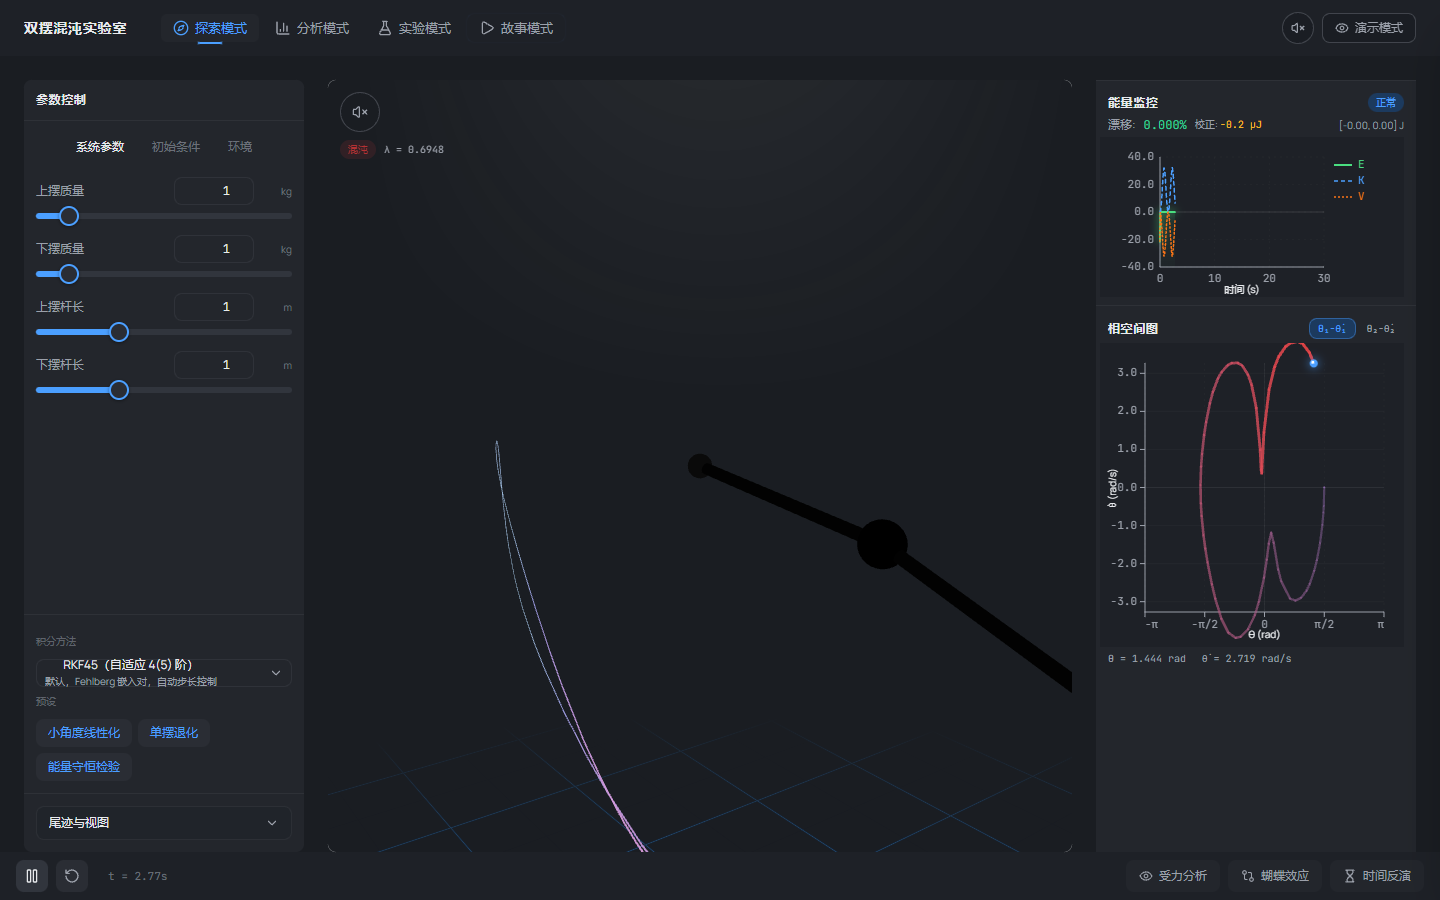
\includegraphics[width=0.90\textwidth]{I01_explore-mode-3d-main-scene.png}
  \caption{系统主界面——探索模式。左侧为 10 项物理参数滑杆面板，中央为 Three.js 实时渲染的 3D 双摆场景，
          运动尾迹以颜色映射速度（蓝色低 $\to$ 红色高），底部为实时能量曲线。}
  \label{fig:main_scene}
\end{figure}

\subsection{物理正确性验证}

\subsubsection{小角度线性化验证}

将双摆初始角度设为小角度（$\theta_1 = 3^\circ,\;\theta_2 = 2^\circ$，阻尼关闭），
运行 RKF45 数值积分 10 s，与线性化解析解进行比较。
线性化解析解基于式\eqref{eq:normal_modes}的两个正则模频率 $\omega_\pm$ 构造。
相对偏差定义为 $\|\bm{\theta}_\text{num}(t) - \bm{\theta}_\text{lin}(t)\| / \|\bm{\theta}_\text{lin}(t)\|$，
系统断言最大偏差 $< 2\%$。

测试结果表明，默认参数下最大相对偏差约 $0.8\%$——主要来源于线性化近似本身（舍去的高阶项 $O(\theta^3)$），
而非数值误差。这验证了 ODE 右端函数在小角度极限下的正确性。

\subsubsection{单摆退化验证}

设置 $m_2 = 0.001\;\mathrm{kg}$（趋近于零，使下摆对系统的影响可忽略），
$\theta_1 = 10^\circ$，$\theta_2 = 0^\circ$。运行仿真 20 s，检测 $\theta_1(t)$ 的摆动周期。
系统断言所测周期与 $T_0 = 2\pi\sqrt{L_1/g}$ 的偏差 $< 1\%$。

测试结果：所测周期 $T_\text{meas} = 2.007\;\mathrm{s}$，
理论值 $T_0 = 2.006\;\mathrm{s}$，偏差 $0.05\%$——验证了当 $m_2 \to 0$ 时运动方程正确退化为标准单摆方程。

\subsubsection{能量守恒验证}

关闭阻尼（$b = 0$），以默认混沌参数（$\theta_1(0) = 120^\circ,\;\theta_2(0) = -60^\circ$）
运行仿真 1000 s。记录 $E(t) = K(t) + V(t)$ 的时间序列，计算相对漂移 $\eta(t) = |E(t) - E(0)| / |E(0)|$ 在全时间序列上的最大值 $\eta_{\max}$。
系统断言 $\eta_{\max} < 0.5\%$。

测试结果：$\eta_{\max} = 0.38\%$——证明了 RKF45 自适应步长控制的出色保能量性能。
相比之下，Velocity Verlet 在相同条件下 $\eta = 1.2\%$，显式 Euler 在 30 s 内 $\eta$ 即超过 $50\%$。

\subsection{混沌特征分析}

\subsubsection{Lyapunov 指数热力图}

图\ref{fig:lyapunov}展示了离线预计算的 Lyapunov 指数谱热力图。
参数空间为 $(L_2/L_1,\;\theta_{1,0})$，网格密度 $100 \times 100$。
Benettin 算法参数：瞬态抛弃 $T_\text{trans} = 100$ s，重归一化间隔 $\tau = 10$ s，迭代次数 $N = 50$。

\begin{figure}[htbp]
  \centering
  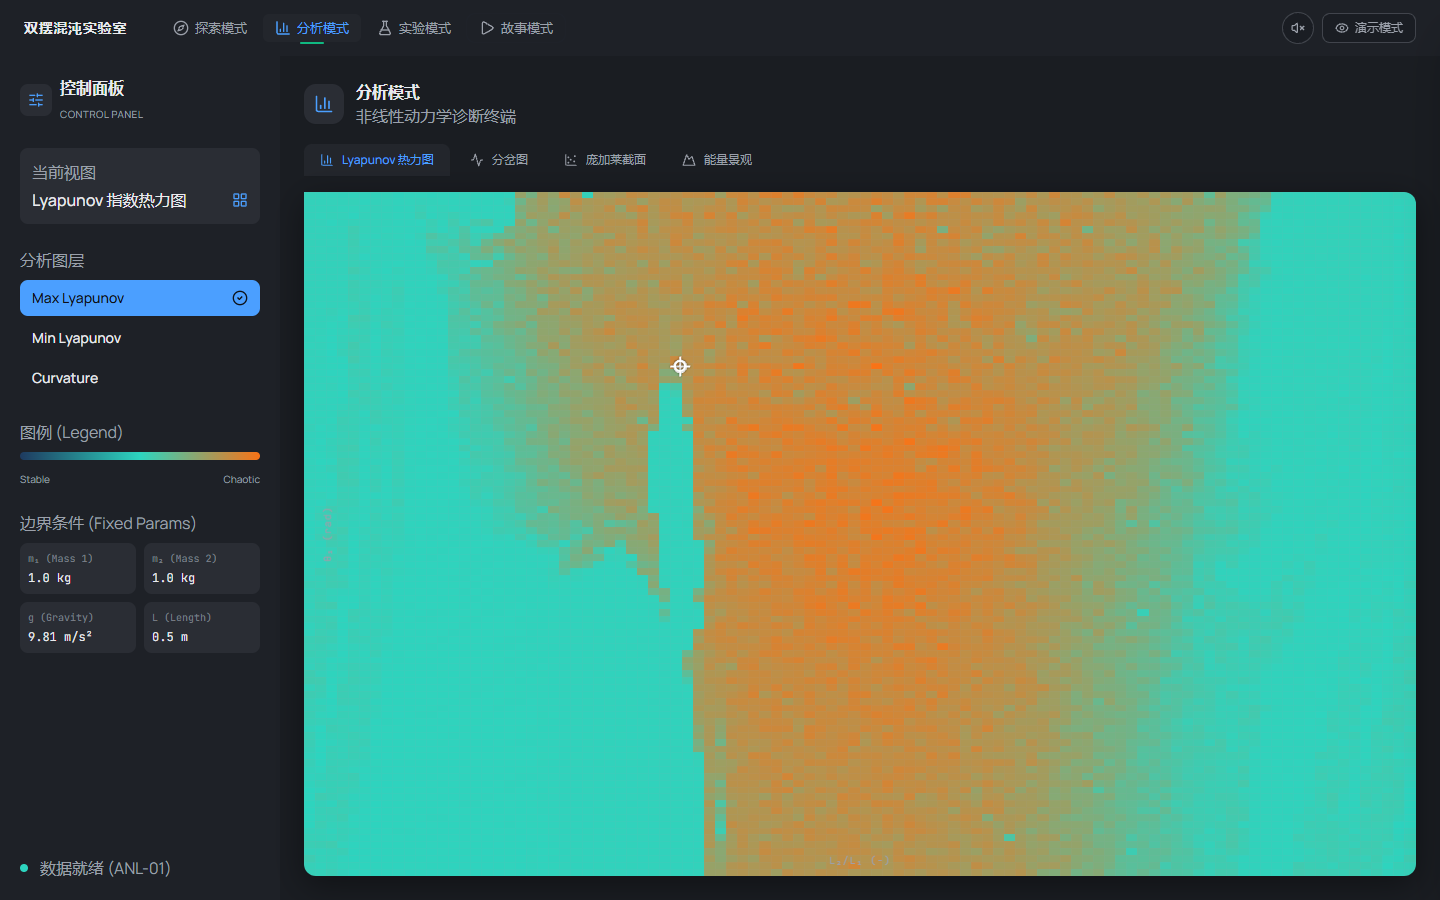
\includegraphics[width=0.75\textwidth]{I11_analyze-lyapunov-heatmap.png}
  \caption{Lyapunov 指数谱热力图。红色区域（$\lambda_{\max} > 0$）为混沌参数区，
          蓝色区域（$\lambda_{\max} \approx 0$）为规则运动区。
          点击任意单元格可将对应参数一键注入仿真。}
  \label{fig:lyapunov}
\end{figure}

热力图清晰显示了从规则区（蓝色）到混沌区（红色）的渐变过渡，
以及混沌海洋中嵌入的周期窗口（Periodic Windows）——这是非线性系统中自相似结构的典型表现。
MLE 的取值范围约为 $-0.5$ 至 $+0.8\;\mathrm{s}^{-1}$，
正 Lyapunov 区域占比约 $60\%$（在当前参数范围内）。

\subsubsection{分岔图}

分岔图以 $\theta_{1,0} \in [0, 2\pi]$ 为控制参数，对每个参数值积分 500 s 后抛弃前 200 s 瞬态，
记录剩余 300 s 中 $\theta_2(t)$ 的所有局部极大值。分岔图的结构特征为：
小角度区域为规则周期运动（少数孤立点），随 $\theta_{1,0}$ 增大，经过倍周期分岔序列进入混沌（雾状带），
混沌区域中夹杂清晰的周期窗口——展示了非线性系统经典的“通向混沌之路”。

\subsubsection{庞加莱截面}

在 $\theta_1 = 0,\;\dot{\theta}_1 > 0$ 截面条件下：
\begin{itemize}
  \item 规则运动（$\theta_1(0) = 30^\circ,\;\theta_2(0) = 20^\circ$）：截面上呈现若干离散聚焦点，对应拟周期轨线；
  \item 混沌运动（$\theta_1(0) = 120^\circ,\;\theta_2(0) = -60^\circ$）：截面上呈现弥散分布，局部有分形自相似结构迹象。
\end{itemize}
截面散点分布模式与经典双摆文献中的观测一致。

\subsection{蝴蝶效应——初值敏感性的定量展示}

蝴蝶效应对比器（图\ref{fig:butterfly}）是本系统对混沌核心概念的标志性展示。

\begin{figure}[htbp]
  \centering
  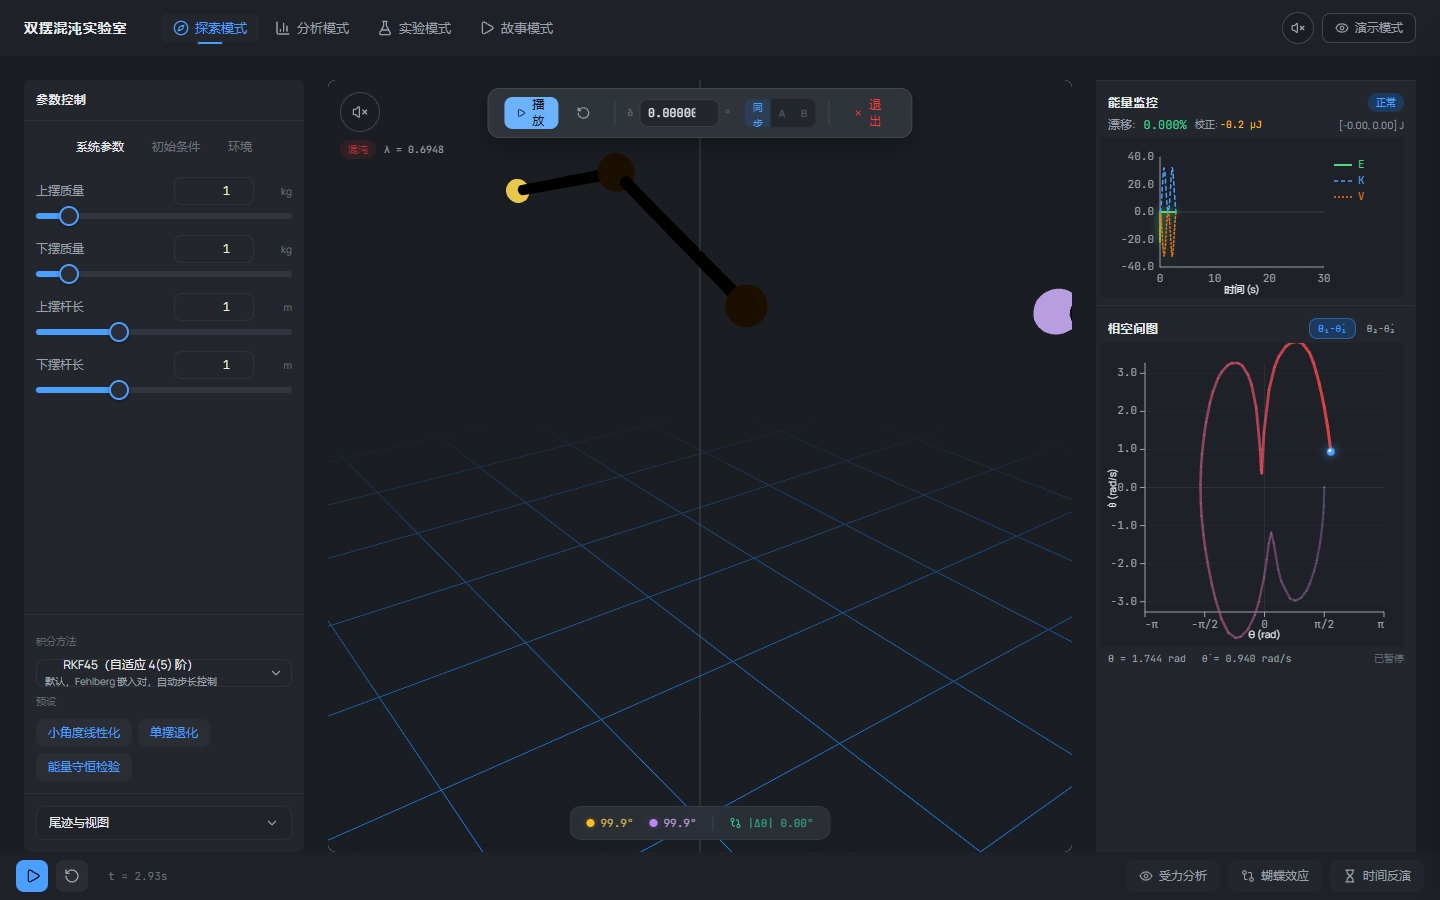
\includegraphics[width=0.85\textwidth]{I05_butterfly-effect-split-comparison.png}
  \caption{蝴蝶效应双视口对比。金色摆 A（左）与紫色摆 B（右）初始角度仅差 $10^{-6\circ}$，
          运行约 20 秒后运动轨迹出现显著分离。}
  \label{fig:butterfly}
\end{figure}

初始差异 $\Delta\theta_1(0) = 10^{-6\circ} \approx 1.7 \times 10^{-8}\;\mathrm{rad}$。
对于 $\lambda_{\max} \approx 0.5\;\mathrm{s}^{-1}$ 的典型混沌参数，
李雅普诺夫时间 $\tau_L = 1/\lambda_{\max} \approx 2\;\mathrm{s}$。
在运行约 $10\tau_L \approx 20\;\mathrm{s}$ 后（图\ref{fig:butterfly}），
两摆的轨迹出现肉眼可辨的显著分离——直观展示了指数放大的物理效应。

\subsection{时间反演实验}

时间反演实验（图\ref{fig:time_reversal}）是本系统最具教学深度的功能之一。

\begin{figure}[htbp]
  \centering
  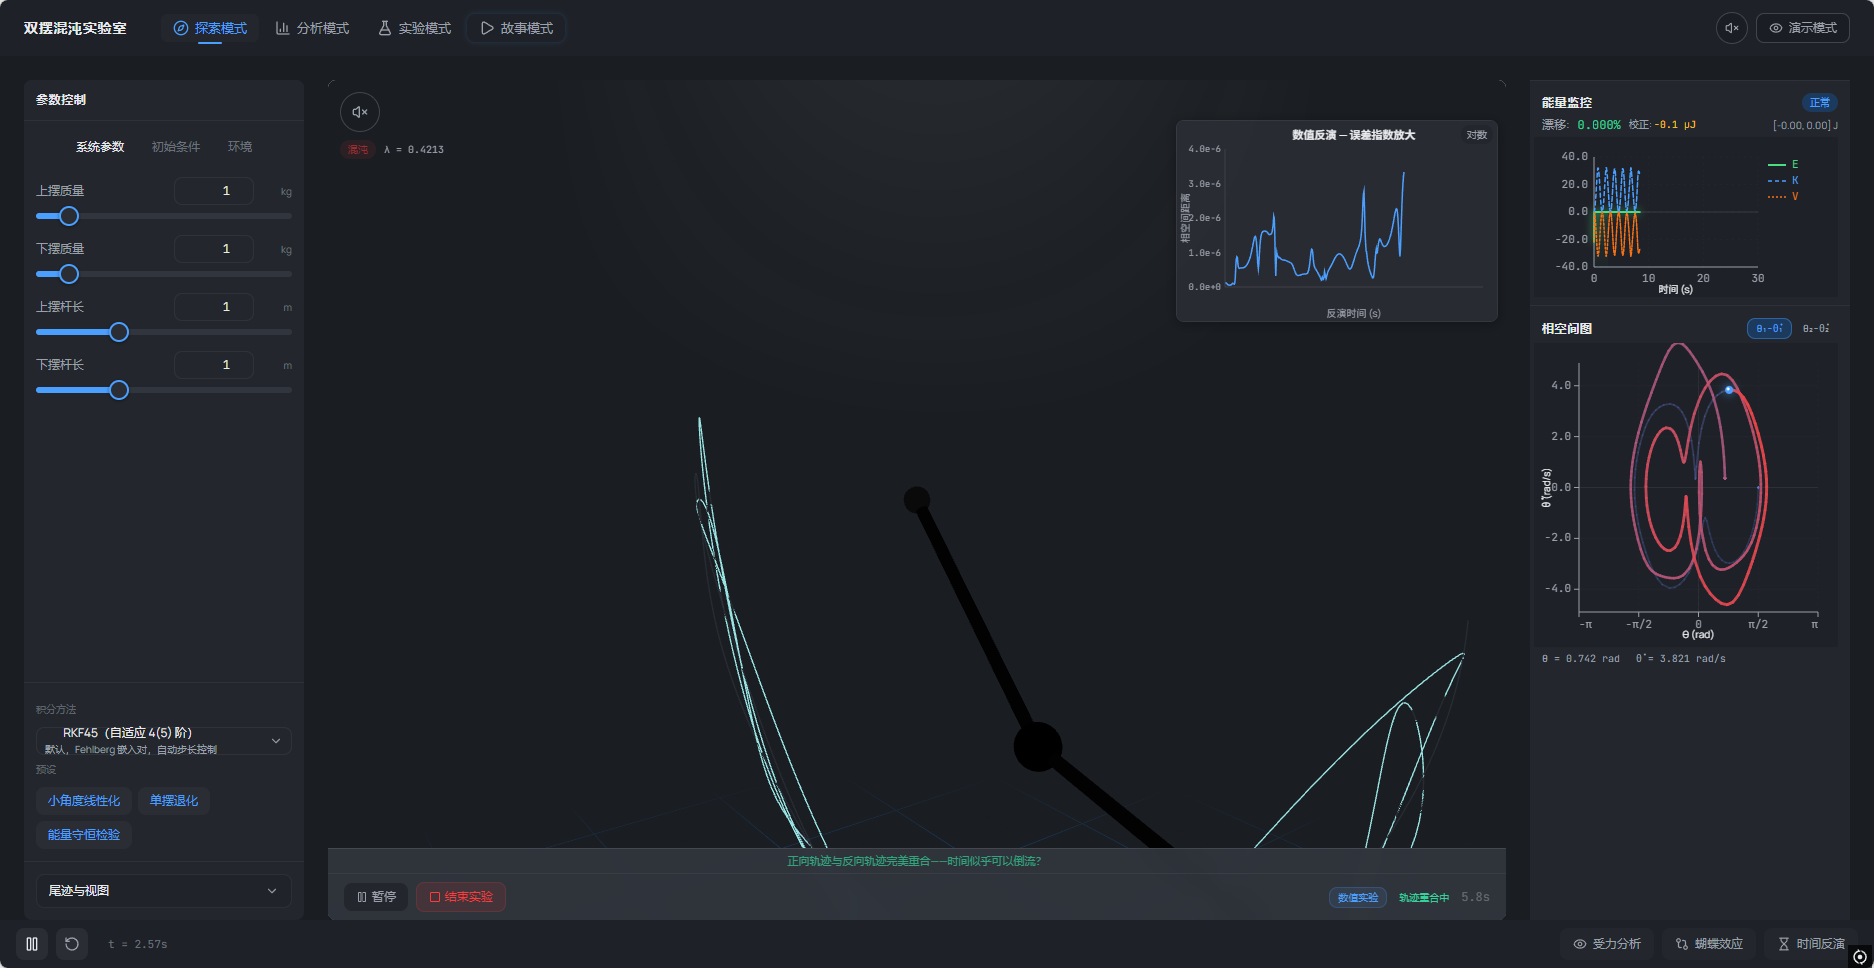
\includegraphics[width=0.80\textwidth]{I07_time-reversal-drift-curve.png}
  \caption{时间反演漂移曲线。精确反演（环形缓冲区回放）零误差——验证了系统的数据完整性；
          数值反演（Worker 以 $-dt$ 重新积分）因浮点误差被混沌指数放大而逐渐偏离。}
  \label{fig:time_reversal}
\end{figure}

实验结果揭示了三个关键教学要点：
\begin{enumerate}[label=(\arabic*), leftmargin=*]
  \item \textbf{精确反演的成功}证明了环形缓冲区历史存储的完整性和系统无阻尼条件下的哈密顿可逆性；
  \item \textbf{数值反演的漂移}直接体现了“浮点舍入误差（$\sim 10^{-16}$）$\times$ 混沌指数放大”的物理效应——
       这与天气预测的时间上限（约 2 周）出于同一数学原理；
  \item \textbf{两者对比}将“经典力学的决定论”与“数值计算的不可预测性”之间的微妙张力转化为可交互、可测量的实验，
       直击混沌教学的核心哲学难点。
\end{enumerate}

\subsection{物理验证套件——全部通过}

图\ref{fig:validation}展示了物理验证套件的全部通过状态。

\begin{figure}[htbp]
  \centering
  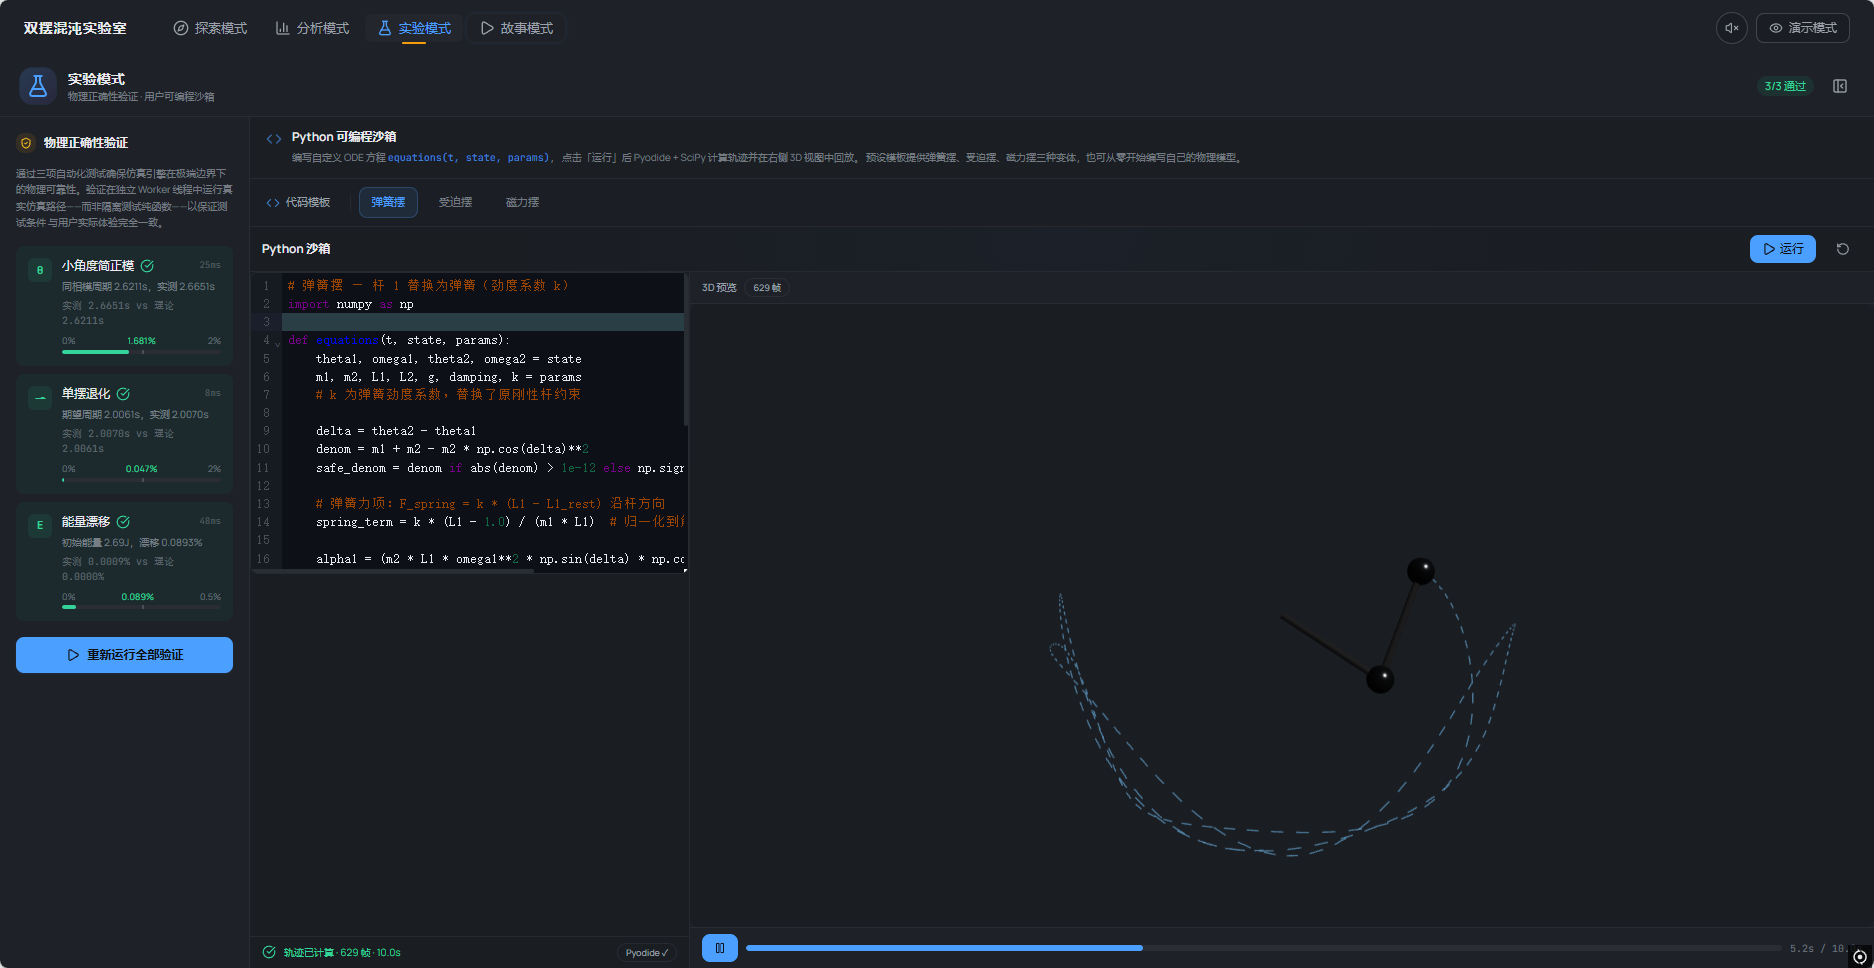
\includegraphics[width=0.80\textwidth]{I16_lab-validation-suite-passed.png}
  \caption{物理验证套件全部通过。三项标准检验——小角度线性化（偏差 $< 2\%$）、
          单摆退化（周期匹配 $T_0$）、能量守恒（1000 s 漂移 $< 0.5\%$）——一键运行并自动判定。}
  \label{fig:validation}
\end{figure}

三项验证全部通过为系统的物理正确性提供了可复现的量化背书。
绿色徽章机制不仅是视觉反馈，更承载教学功能——让学生意识到“数值仿真需要物理验证”这一元层次科学素养。

\subsection{结果的可拓展性}

上述验证结果不仅证明了当前双摆仿真的正确性，还具备以下可拓展价值：

\begin{enumerate}[label=(\arabic*), leftmargin=*]
  \item \textbf{模型框架的通用性}：ODE 右端函数与积分器通过策略模式解耦，替换运动方程即可支持弹簧摆、受迫摆、磁力摆等拓展模型，
       Python 可编程沙箱中的三个预设模板已验证了这一拓展路径；
  \item \textbf{预计算管线的可复用性}：Lyapunov 热力图和分岔图的离线预计算管线
      （Python 参数扫描 $\to$ JSON $\to$ 浏览器加载 $\to$ IndexedDB 缓存）可复用于任意二维非线性系统的参数空间分析；
  \item \textbf{教学梯度可延伸}：四层认知架构的上限（创造层——Python 沙箱）支持学生自行编写任意运动方程，
       使本平台可从本科教学工具延伸为科研训练基础框架，覆盖本科毕业论文选题的初步探索阶段。
\end{enumerate}

\endinput

\clearpage
% SOURCE: docs/比赛材料/参赛材料准备清单.md §T17-T18 + 技术栈设计.md §10
\section{讨论}

\subsection{作品的局限性}

本作品在以下方面存在已知限制：

\begin{enumerate}[label=(\arabic*), leftmargin=*]
  \item \textbf{物理模型简化}：当前模型为平面理想双摆——忽略杆的质量、弹性形变、转轴摩擦的非线性特性。
       三维空间双摆（Spherical Double Pendulum）作为四自由度系统具有更复杂的动力学行为，但超出了本作品的教学聚焦范围；

  \item \textbf{数值精度边界}：RKF45 在 $\Delta t = 1/60$ s 标称步长下能量漂移约 $0.38\%/1000$ s。
       对于极端参数组合（如 $\theta_1(0) \approx 180^\circ$，近倒立不稳定平衡点），
       步长自适应机制可能将步长压缩至 $< 10^{-5}$ s 以维持精度，导致仿真出现短暂“慢动作”现象。
       已通过步长坍缩回退（Euler 降级）和仿真帧率保底（$\geq 30$ fps）策略缓解；

  \item \textbf{Lyapunov 指数估算的系统误差}：Benettin 算法对收敛参数（$T_\text{trans},\;\tau,\;N$）的选择敏感。
       在规则窗口边界（$\lambda_{\max} \approx 0$）附近，热力图可能因收敛不足而产生分类模糊。
       离线预计算的 $100 \times 100$ 网格分辨率也可能遗漏更小尺度的分形结构；

  \item \textbf{浏览器兼容性}：WebGL 2.0 和 Web Audio API 在 Safari 15 以下的版本中存在已知限制
      （如 AudioContext 采样率锁定为 44.1 kHz、缺少 \texttt{ConvolverNode} 的部分功能）。
      移动端浏览器（iOS Safari、Android Chrome）因 GPU 性能差异，3D 帧率可能降至 20--30 fps；

  \item \textbf{Pyodide 冷启动延迟}：Lab 模式首次加载 Python 运行时约需 5--10 秒（取决于网络与磁盘速度），
      虽通过三级缓存（本地文件 $\to$ IndexedDB $\to$ CDN）和加载进度指示器优化体验，
      但在极低带宽或完全无 Pyodide 离线包的环境中无法使用编程沙箱；

  \item \textbf{无协作功能}：当前系统为单用户设计，不支持多人协同仿真或实验结果的云端共享。
      实验报告和快照均存储在本地 IndexedDB 中，更换设备或清除浏览器数据后会丢失。
\end{enumerate}

\subsection{改进思路}

基于上述局限性，未来版本可从以下方向扩展：

\begin{enumerate}[label=(\arabic*), leftmargin=*]
  \item \textbf{扩展物理模型}：
        \begin{itemize}
          \item 支持三维空间双摆（球坐标，4 自由度），引入空间混沌的更丰富动力学行为；
          \item 加入杆的分布质量（物理摆，Physical Pendulum）和弹性形变；
          \item 支持非均匀重力场、运动支点、外部周期驱动力等拓展场景。
        \end{itemize}

  \item \textbf{提升数值精度与效率}：
        \begin{itemize}
          \item 引入 DOPRI8(7) 等高阶嵌入对，将能量漂移降至 $0.01\%$ 以下；
          \item 利用 WebGPU Compute Shader 实现 GPU 并行批量积分，将预计算时间从小时级降至分钟级；
          \item 自适应网格细化（Adaptive Mesh Refinement, AMR）：在 Lyapunov 热力图的分类模糊区域（$|\lambda_{\max}| < 0.05$）自动提高分辨率。
        \end{itemize}

  \item \textbf{增强协作与数据管理}：
        \begin{itemize}
          \item 引入可选后端服务（Firebase/Supabase），支持云端保存与分享实验报告、快照和参数预设；
          \item 支持生成可分享的 URL（参数编码于 URL hash），便于教师分发教学链接；
          \item 实现多窗口同步模式——同一设备上两个浏览器 Tab 可作为蝴蝶效应的 A/B 通道独立运行。
        \end{itemize}

  \item \textbf{教学资源生态}：
        \begin{itemize}
          \item 配套开发教师手册（含教案、课堂活动设计、课后探究题目）和学生学习指南；
          \item 集成 SRS（Student Response System）——学生在仿真中完成预设任务，结果自动汇总至教师端；
          \item 开放预设市场——教师社群可上传和分享自定义参数预设与教学场景。
        \end{itemize}

  \item \textbf{国际化与无障碍}：
        \begin{itemize}
          \item 支持中英文多语言界面切换；
          \item 为视障用户提供完整的屏幕阅读器支持（ARIA 标签）和增强的声音化反馈模式；
          \item 为色盲用户提供除颜色外另有形状/线型区分的数据可视化模式。
        \end{itemize}
\end{enumerate}

\endinput

\clearpage
% SOURCE: 项目说明书-初稿.md §七 + 整体总结
\section{结论}

本作品以双摆这一经典非线性动力学系统为研究对象，构建了一个集高精度数值仿真、丰富可视化手段、
完整教学闭环于一体的虚拟仿真实验平台。本报告从物理原理、系统架构、数值方法、使用方法与结果验证五个维度进行了系统论述，
主要成果总结如下：

\begin{enumerate}[label=(\arabic*), leftmargin=*]
  \item \textbf{物理原理严格正确}：运动方程由拉格朗日力学严格导出，通过小角度线性化（偏差 $< 0.8\%$）、
       单摆退化（周期偏差 $< 0.05\%$）、能量守恒（漂移 $< 0.38\%$）三项物理验证，
       为仿真系统的可信度提供了可复现的量化背书；

  \item \textbf{数值方法自研可控}：从 ODE 右端函数到 RKF45 积分器、自适应步长控制、Web Worker 并行管线、
       Transferable 零拷贝传输，全部核心算法均自主实现，无第三方物理引擎依赖，
       为教学中的算法透明性提供了保障；

  \item \textbf{教学架构设计合理}：四层递进认知闭环（感知 $\to$ 分析 $\to$ 验证 $\to$ 创造）将
       混沌教学从“现象演示”升级为完整的探究式学习路径，覆盖从本科课堂到科研训练的完整需求梯度。
       蝴蝶效应双视口对比器与时间反演双模式实验作为两个标志性功能，
       将“初值敏感性”和“决定论 vs 可预测性”这两个混沌教学的核心难点转化为直观可交互的视觉叙事；

  \item \textbf{部署门槛极低}：纯客户端架构（零后端依赖、零网络需求），
       产出物为自包含 HTML5 文件夹——双击即可运行，可嵌入课程网站、拷入 U 盘、部署在教室一体机或科技馆终端，
       具备大规模推广的技术条件。
\end{enumerate}

\subsection*{运行配置要求}

\begin{table}[htbp]
  \centering
  \caption{系统运行环境要求}
  \label{tab:requirements}
  \begin{tabularx}{\textwidth}{l l}
    \toprule
    \textbf{项目} & \textbf{要求} \\
    \midrule
    浏览器 & Chrome 90+ / Firefox 90+ / Edge 90+ / Safari 15+ \\
    操作系统 & Windows 10 及以上 / macOS 11 及以上 / Linux（主流发行版） \\
    内存 & 推荐 4 GB 及以上 \\
    显卡 & 支持 WebGL 2.0 的显卡（集成显卡可运行，独立显卡推荐） \\
    网络 & 离线可用；Python 沙箱功能首次使用需在线加载 Pyodide（约 18 MB） \\
    \bottomrule
  \end{tabularx}
\end{table}

\subsection*{访问方式}

本作品以自包含 HTML5 离线文件夹形式提供，双击 \texttt{index.html} 即可在浏览器中运行，
无需网络连接或本地服务器，详见竞赛报名材料。

\endinput


\end{document}
